\documentclass[12pt, a4paper, oneside]{ctexart}
\usepackage{amsmath, amsthm, amssymb, bm, color, graphicx, geometry, mathrsfs,extarrows, braket, booktabs, array, wrapfig, enumitem, subfigure}
\usepackage[colorlinks,linkcolor=red,anchorcolor=blue,citecolor=blue,urlcolor=blue,menucolor=black]{hyperref}
%%%% 设置中文字体 %%%%
% fc-list -f "%{family}\n" :lang=zh >d:zhfont.txt 命令查看已有字体
\setCJKmainfont{方正书宋.ttf}[BoldFont = 方正黑体_GBK.ttf, ItalicFont = simkai.ttf, BoldItalicFont = 方正粗楷简体.ttf]
%%%% 设置英文字体 %%%%
\setmainfont{Times New Roman}
\setsansfont{Calibri}
\setmonofont{Consolas}

%%%% 设置代码块 %%%%
% 在vscode中使用minted需要先配置python解释器, Ctrl+Shift+P, 输入Python: Select Interpreter选择安装了Pygments的Python版本. 再在setting.json中xelatex和pdflatex的参数中加入 "--shell-escape", 即可
% TeXworks中配置方法参考: https://blog.csdn.net/RobertChenGuangzhi/article/details/108140093
\usepackage{minted}
\renewcommand{\theFancyVerbLine}{
    \sffamily\textcolor[rgb]{0.5,0.5,0.5}{\scriptsize\arabic{FancyVerbLine}}} % 修改代码前序号大小
% 加入不同语言的代码块
\newmintinline{cpp}{fontsize=\small, linenos, breaklines, frame=lines}
\newminted{cpp}{fontsize=\small, baselinestretch=1, linenos, breaklines, frame=lines}
\newmintedfile{cpp}{fontsize=\small, baselinestretch=1, linenos, breaklines, frame=lines}
\newminted{r}{fontsize=\small, baselinestretch=1, linenos, breaklines, frame=lines}
\newmintinline{matlab}{fontsize=\small, linenos, breaklines, frame=lines}
\newminted{matlab}{fontsize=\small, baselinestretch=1, mathescape, linenos, breaklines, frame=lines}
\newmintedfile{matlab}{fontsize=\small, baselinestretch=1, linenos, breaklines, frame=lines}
\newmintinline{python}{fontsize=\small, linenos, breaklines, frame=lines, python3}  % 使用\pythoninline{代码}
\newminted{python}{fontsize=\small, baselinestretch=1, linenos, breaklines, frame=lines, python3}  % 使用\begin{pythoncode}代码\end{pythoncode}
\newmintedfile{python}{fontsize=\small, baselinestretch=1, linenos, breaklines, frame=lines, python3}  % 使用\pythonfile{代码地址}

%%%% 设置行间距与页边距 %%%%
\linespread{1.4}
%\geometry{left=2.54cm,right=2.54cm,top=3.18cm,bottom=3.18cm}
\geometry{left=1.84cm,right=1.84cm,top=2.18cm,bottom=2.18cm}

%%%% 图片相对路径 %%%%
\graphicspath{{figures/}} % 当前目录下的figures文件夹, {../figures/}则是父目录的figures文件夹
\setlength{\abovecaptionskip}{-0.2cm}  % 缩紧图片标题与图片之间的距离
\setlength{\belowcaptionskip}{0pt} 

%%%% 缩小item,enumerate,description两行间间距 %%%%
\setenumerate[1]{itemsep=0pt,partopsep=0pt,parsep=\parskip,topsep=5pt}
\setitemize[1]{itemsep=0pt,partopsep=0pt,parsep=\parskip,topsep=5pt}
\setdescription{itemsep=0pt,partopsep=0pt,parsep=\parskip,topsep=5pt}

%%%% 自定义公式 %%%%
\everymath{\displaystyle} % 默认全部行间公式
\DeclareMathOperator*\uplim{\overline{lim}} % 定义上极限 \uplim_{}
\DeclareMathOperator*\lowlim{\underline{lim}} % 定义下极限 \lowlim_{}
\DeclareMathOperator*{\argmax}{arg\,max}  % 定义取最大值的参数 \argmax_{}
\DeclareMathOperator*{\argmin}{arg\,min}  % 定义取最小值的参数 \argmin_{}
\let\leq=\leqslant % 将全部leq变为leqslant
\let\geq=\geqslant % geq同理
\DeclareRobustCommand{\rchi}{{\mathpalette\irchi\relax}}
\newcommand{\irchi}[2]{\raisebox{\depth}{$#1\chi$}} % 使用\rchi将\chi居中

%%%% 自定义环境配置 %%%%
\newcounter{problem}  % 问题序号计数器
\newenvironment{problem}[1][]{\stepcounter{problem}\par\noindent\textbf{题目\arabic{problem}. #1}}{\smallskip\par}
\newenvironment{solution}[1][]{\par\noindent\textbf{#1解答. }}{\smallskip\par}  % 可带一个参数表示题号\begin{solution}{题号}
\newenvironment{note}{\par\noindent\textbf{注记. }}{\smallskip\par}
\newenvironment{remark}{\begin{enumerate}[label=\textbf{注\arabic*.}]}{\end{enumerate}}
\BeforeBeginEnvironment{minted}{\vspace{-0.5cm}}  % 缩小minted环境距上文间距
\AfterEndEnvironment{minted}{\vspace{-0.2cm}}  % 缩小minted环境距下文间距

%%%% 一些宏定义 %%%%
\def\bd{\boldsymbol}        % 加粗(向量) boldsymbol
\def\disp{\displaystyle}    % 使用行间公式 displaystyle(默认)
\def\weekto{\rightharpoonup}% 右半箭头
\def\tsty{\textstyle}       % 使用行内公式 textstyle
\def\sign{\text{sign}}      % sign function
\def\wtd{\widetilde}        % 宽波浪线 widetilde
\def\R{\mathbb{R}}          % Real number
\def\N{\mathbb{N}}          % Natural number
\def\Z{\mathbb{Z}}          % Integer number
\def\Q{\mathbb{Q}}          % Rational number
\def\C{\mathbb{C}}          % Complex number
\def\K{\mathbb{K}}          % Number Field
\def\P{\mathbb{P}}          % Polynomial
\def\d{\mathrm{d}}          % differential operator
\def\e{\mathrm{e}}          % Euler's number
\def\i{\mathrm{i}}          % imaginary number
\def\re{\mathrm{Re}}        % Real part
\def\im{\mathrm{Im}}        % Imaginary part
\def\res{\mathrm{Res}}      % Residue
\def\ker{\mathrm{Ker}}      % Kernel
\def\vspan{\mathrm{vspan}}  % Span  \span与latex内核代码冲突改为\vspan
\def\L{\mathcal{L}}         % Loss function
\def\O{\mathcal{O}}         % big O notation
\def\wdh{\widehat}          % 宽帽子 widehat
\def\ol{\overline}          % 上横线 overline
\def\ul{\underline}         % 下横线 underline
\def\add{\vspace{1ex}}      % 增加行间距
\def\del{\vspace{-1.5ex}}   % 减少行间距

%%%% 定理类环境的定义 %%%%
\newtheorem{theorem}{定理}

%%%% 基本信息 %%%%
\newcommand{\RQ}{\today} % 日期
\newcommand{\km}{数据分析} % 科目
\newcommand{\bj}{强基数学002} % 班级
\newcommand{\xm}{吴天阳} % 姓名
\newcommand{\xh}{2204210460} % 学号

\begin{document}

%\pagestyle{empty}
\pagestyle{plain}
\vspace*{-15ex}
\centerline{\begin{tabular}{*5{c}}
    \parbox[t]{0.25\linewidth}{\begin{center}\textbf{日期}\\ \large \textcolor{blue}{\RQ}\end{center}} 
    & \parbox[t]{0.2\linewidth}{\begin{center}\textbf{科目}\\ \large \textcolor{blue}{\km}\end{center}}
    & \parbox[t]{0.2\linewidth}{\begin{center}\textbf{班级}\\ \large \textcolor{blue}{\bj}\end{center}}
    & \parbox[t]{0.1\linewidth}{\begin{center}\textbf{姓名}\\ \large \textcolor{blue}{\xm}\end{center}}
    & \parbox[t]{0.15\linewidth}{\begin{center}\textbf{学号}\\ \large \textcolor{blue}{\xh}\end{center}} \\ \hline
\end{tabular}}
\begin{center}
    \zihao{3}\textbf{第一章作业}
\end{center}\vspace{-0.2cm}
\begin{solution}[1.4]
    \begin{cppcode}
x1: 均值 = 19.16645, 方差 = 392.0308, 标准差 = 19.79977, 变异系数 = 103.3043, 偏度 = 2.391967, 峰度 = 9.804995
x2: 均值 = 246.1932, 方差 = 54276, 标准差 = 232.9721, 变异系数 = 94.62978, 偏度 = 1.821974, 峰度 = 6.521676
x1: 上四分位数 = 8.265, 中位数 = 14.77, 下四分位数 = 20.08
x2: 上四分位数 = 105.35, 中位数 = 179.41, 下四分位数 = 270.745
Pearson相关系数 = 0.9762474, Spearman相关系数 = 0.9278226
    \end{cppcode}
    %%%% 两组图并排放(可溢出一些) %%%%
    \begin{figure}[htbp]
        \vspace{-0.5cm}
        \hspace{-2.5cm}
        \subfigure  % 子图的标题
        {
            % 如果一行放三个图改成0.3\linewidth即可
            \begin{minipage}[b]{.62\linewidth}
                \centering
                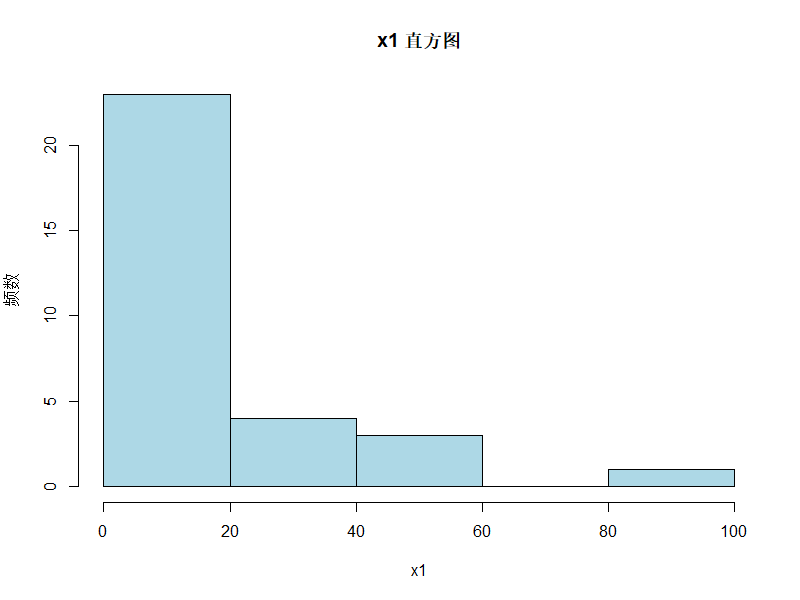
\includegraphics[scale=0.5]{./code/x1_histogram.png}
            \end{minipage}
        }
        \subfigure
        {
            \begin{minipage}[b]{.2\linewidth}
                \centering
                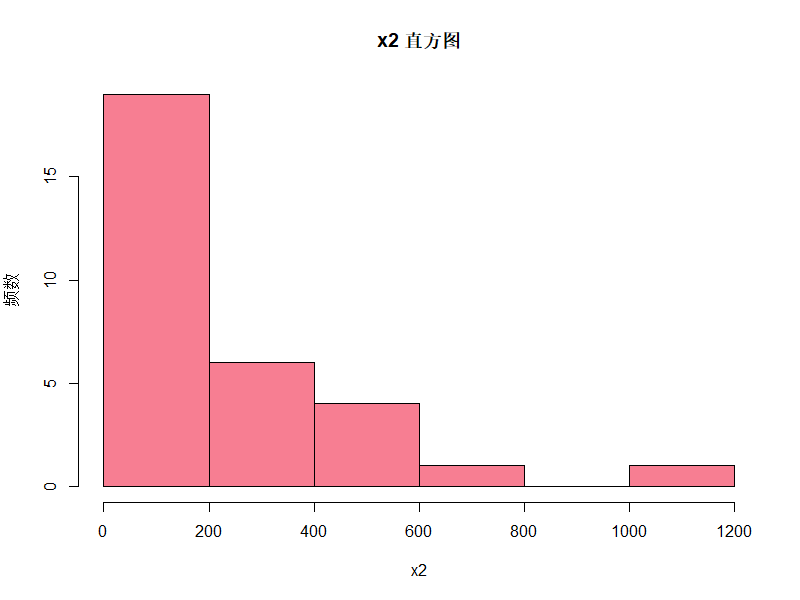
\includegraphics[scale=0.5]{./code/x2_histogram.png}
            \end{minipage}
        }
    \end{figure}
    \begin{figure}[htbp]
        \vspace{-1cm}
        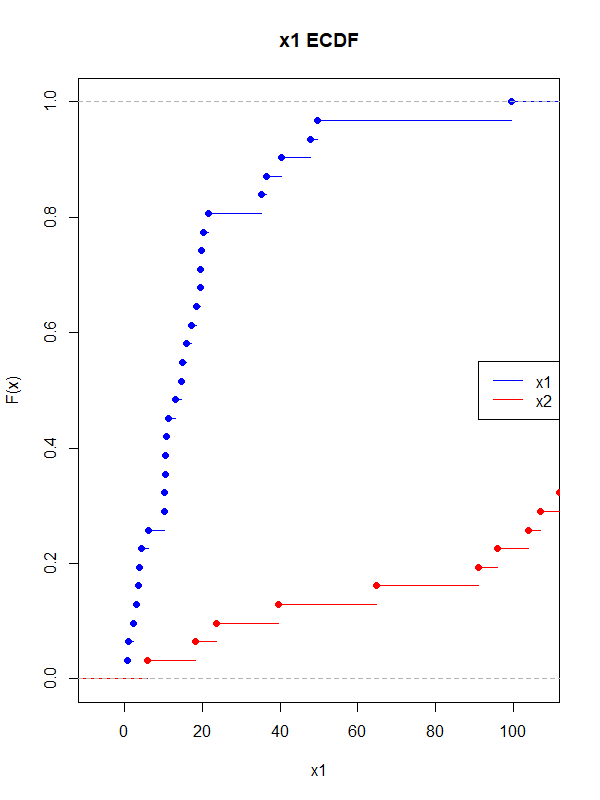
\includegraphics[scale=0.5]{./code/ecdf.png}
    \end{figure}
\end{solution}
\clearpage
\begin{solution}[1.5]
    均值向量为
    \begin{cppcode}
       V1        V2        V3        V4
18.219048 27.866667  4.504762 33.766667
    \end{cppcode}
    协方差矩阵为
    \begin{cppcode}
         V1       V2       V3       V4
V1 3.508619 2.707167 1.019405 1.265667
V2 2.707167 3.559333 1.138667 1.289333
V3 1.019405 1.138667 1.998476 1.739667
V4 1.265667 1.289333 1.739667 4.032333
    \end{cppcode}
\end{solution}
\begin{solution}[1.6]
\begin{cppcode}
中位数向量
  V1   V2   V3   V4
18.1 27.4  4.8 34.1

Pearson相关矩阵
          V1        V2        V3        V4
V1 1.0000000 0.7660596 0.3849719 0.3364907
V2 0.7660596 1.0000000 0.4269360 0.3403319
V3 0.3849719 0.4269360 1.0000000 0.6128276
V4 0.3364907 0.3403319 0.6128276 1.0000000

Spearman相关矩阵
          V1        V2        V3        V4
V1 1.0000000 0.7896983 0.4339915 0.4305367
V2 0.7896983 1.0000000 0.5111078 0.4884056
V3 0.4339915 0.5111078 1.0000000 0.6911813
V4 0.4305367 0.4884056 0.6911813 1.0000000

Pearson检验
             [,1]          [,2]          [,3]        [,4]
[1,] 0.000000e+00  5.152838e-05  8.483807e-02 0.135839682
[2,] 5.152838e-05 3.532105e-150  5.357904e-02 0.131150557
[3,] 8.483807e-02  5.357904e-02 3.532105e-150 0.003140558
[4,] 1.358397e-01  1.311506e-01  3.140558e-03 0.000000000

Spearman检验
             [,1]         [,2]         [,3]          [,4]
[1,] 0.000000e+00 2.070355e-05 0.0493361598  5.138011e-02
[2,] 2.070355e-05 0.000000e+00 0.0178878482  2.467570e-02
[3,] 4.933616e-02 1.788785e-02 0.0000000000  5.210014e-04
[4,] 5.138011e-02 2.467570e-02 0.0005210014 2.557517e-147
\end{cppcode}
\end{solution}
\clearpage
\textbf{1.4代码:}
\begin{rcode}
setwd("E:/Coding/R/习题一")
data <- read.table("exercise1_4.txt", fileEncoding = "GB2312")
x1 <- data[, 2]
x2 <- data[, 3]
cat("x1 =", x1, "\nx2 =", x2, "\n")

# 计算均值
mean_x1 <- mean(x1)
mean_x2 <- mean(x2)

# 计算方差
var_x1 <- var(x1)
var_x2 <- var(x2)

# 计算标准差
sd_x1 <- sd(x1)
sd_x2 <- sd(x2)

# 计算变异系数
cv_x1 <- sd_x1 / mean_x1 * 100
cv_x2 <- sd_x2 / mean_x2 * 100

# 计算偏度
skewness_x1 <- moments::skewness(x1)
skewness_x2 <- moments::skewness(x2)

# 计算峰度
kurtosis_x1 <- moments::kurtosis(x1)
kurtosis_x2 <- moments::kurtosis(x2)

# 输出结果
cat("x1: 均值 = ", mean_x1, ", 方差 = ", var_x1, ", 标准差 = ", sd_x1,
    ", 变异系数 = ", cv_x1, ", 偏度 = ", skewness_x1, ", 峰度 = ", kurtosis_x1,
    "\n", sep = "")
cat("x2: 均值 = ", mean_x2, ", 方差 = ", var_x2, ", 标准差 = ", sd_x2,
    ", 变异系数 = ", cv_x2, ", 偏度 = ", skewness_x2, ", 峰度 = ", kurtosis_x2,
    "\n", sep = "")


# 计算上下四分位数及中位数
q1_x1 <- quantile(x1, probs = 0.25)
median_x1 <- quantile(x1, probs = 0.5)
q3_x1 <- quantile(x1, probs = 0.75)

q1_x2 <- quantile(x2, probs = 0.25)
median_x2 <- quantile(x2, probs = 0.5)
q3_x2 <- quantile(x2, probs = 0.75)

# 计算四分位极差
iqr_x1 <- q3_x1 - q1_x1
iqr_x2 <- q3_x2 - q1_x2

cat("x1: 上四分位数 = ", q1_x1, ", 中位数 = ", median_x1, ", 下四分位数 = ", q3_x1,
    "\n", sep = "")
cat("x2: 上四分位数 = ", q1_x2, ", 中位数 = ", median_x2, ", 下四分位数 = ", q3_x2,
    "\n", sep = "")

png("x1_histogram.png", width = 800, height = 600, res = 96)
hist(x1, main = "x1 直方图", xlab = "x1", ylab = "频数", col = "lightblue")
dev.off()
png("x2_histogram.png", width = 800, height = 600, res = 96)
hist(x2, main = "x2 直方图", xlab = "x2", ylab = "频数", col = "#f77e92")
dev.off()

# 计算两组样本的ECDF函数
ecdf_x1 <- ecdf(x1)
ecdf_x2 <- ecdf(x2)

# 绘制ECDF图
png("ecdf.png", width = 600, height = 800, res = 96)
plot(ecdf_x1, main = "经验分布函数图", xlab = "x", ylab = "F(x)", col = "blue")
lines(ecdf_x2, col = "red")
legend("right", legend = c("x1", "x2"), col = c("blue", "red"), lty = 1)
dev.off()

# Pearson相关系数和Spearman相关系数
cor_pearson <- cor(x1, x2, method = "pearson")
cor_spearman <- cor(x1, x2, method = "spearman")

cat("Pearson相关系数 = ", cor_pearson, ", Spearman相关系数 = ", cor_spearman,
    "\n", sep = "")
\end{rcode}
\textbf{1.5和1.6代码:}
\begin{rcode}
setwd("E:/Coding/R/习题一")
data <- read.table("exercise1_5.txt")

# 总体均值向量
data_mean <- colMeans(data)
print(data_mean)
# 总体协方差矩阵
data_cov <- cov(data)
print(data_cov)

# 中位数向量
data_median <- apply(data, 2, median)
cat("中位数向量\n")
print(data_median)

# Pearson相关矩阵
R <- cor(data, method = "pearson")
cat("Pearson相关矩阵\n")
print(R)
# Spearman相关矩阵
Q <- cor(data, method = "spearman")
cat("Spearman相关矩阵\n")
print(Q)

# 计算Pearson两两列做相关性分析
pearson_values <- matrix(nrow = ncol(data), ncol = ncol(data))
spearman_values <- matrix(nrow = ncol(data), ncol = ncol(data))
for (j in 1:ncol(data)) {
    for (k in 1:ncol(data)) {
        pearson_test <- cor.test(data[, j], data[, k])
        pearson_values[j, k] <- pearson_test$p.value
        spearman_test <- cor.test(data[, j], data[, k], method = "spearman")
        spearman_values[j, k] <- spearman_test$p.value
    }
}
cat("Pearson检验\n")
print(pearson_values)
cat("Spearman检验\n")
print(spearman_values)
\end{rcode}
\end{document}